% cd /storage/emulated/0/Documents/documents/latex/1920/Grade-10/2nd/equation-and-graph-of-a-circle && pdflatex hand-equation-and-graph-of-a-circle.tex && divide 2x2 hand-equation-and-graph-of-a-circle.pdf


\documentclass[handout]{beamer} 

\usepackage{pgfpages} 
\mode<handout>{%
\pgfpagesuselayout{4 on 1}[
%letterpaper, 
legalpaper, %landscape, 
border shrink=1mm] 
%\setbeameroption{show notes} 
}

\usepackage{xcolor}
\usepackage{anyfontsize}
\usepackage{enumitem}
\usepackage{multicol}
\usepackage{amsmath, makecell}
\usepackage{tabularx} 
\usepackage{gensymb}
\usepackage{wasysym} %for checked symbol 
\usepackage{multirow}
\usepackage{graphicx, tipa}
\usepackage{tikz}
\usetikzlibrary{angles,quotes}
\usepackage{pgfplots} 
\usetikzlibrary{calc}
\pgfplotsset{compat=newest}
\usetikzlibrary{arrows.meta}
\usetikzlibrary{intersections}
\usetikzlibrary{decorations.pathreplacing}
\usepackage{flafter}
%\usepackage{fourier} 
\usepackage{amsmath,amssymb,cancel,units}
\usepackage{microtype} % nicer output 
\usepackage{hfoldsty} % nicer output 
\usepackage{fixltx2e} 
\usepackage{mathptmx}
\usepackage{numprint}
\usepackage[T1]{fontenc}
\usepackage[utf8]{inputenc} 
\usepackage{stackengine} %to define \pesos 
\usepackage{lmodern} %scalable font
\usepackage{booktabs}
\usepackage{array}


\pagenumbering{gobble}
%\linespread{0.9}
\newcommand{\vspce}{\vspace{0.75ex}}

\newcommand{\hspce}{\hspace{0.5em}}

\newcommand{\blank}{\underline{\hspace{2em}}}%{\rule{1em}{0.15ex}}

\newcommand{\arc}[1]{{% 
\setbox9=\hbox{#1}% 
\ooalign{\resizebox{\wd9}{\height}{\texttoptiebar{\phantom{A}}}\cr#1}}}


\newcommand\pesos{\stackengine{-1.4ex}{P}{\stackengine{-1.25ex}{$-$}{$-$}{O}{c}{F}{F}{S}}{O}{c}{F}{T}{S}} 


\renewcommand\theadalign{bc} 

\renewcommand\theadfont{\bfseries} 

\renewcommand\theadgape{\Gape[4pt]} 

\renewcommand\cellgape{\Gape[4pt]} 

\pagenumbering{gobble}

\newcolumntype{Y}{>{\centering\arraybackslash}X} %for tabularx

\newcolumntype{R}{>{\raggedleft\arraybackslash}X} %for tabularx

\newcolumntype{Z}{>{\raggedleft\arraybackslash}X} %for tabularx

\newcolumntype{L}{>{\raggedright\arraybackslash}X} %for tabularx

\newcolumntype{A}[1]{>{\raggedright\arraybackslash}p{#1}} %for longtable LEFT

\newcolumntype{C}[1]{>{\centering\arraybackslash}p{#1}} %for longtable CENTER

\newcolumntype{B}[1]{>{\raggedleft\arraybackslash}p{#1}} %for longtable RIGHT 
 
\renewcommand{\tabularxcolumn}[1]{>{\small}m{#1}}

\newcolumntype{N}[1]{>{\raggedleft}p{#1}} %for tabular left 

\newcolumntype{M}[1]{>{\raggedright\arraybackslash}p{#1}} %for tabular right 

\newcommand{\myaxis}{xticklabels={}, 
yticklabels={}, 
ymin=-10, ymax=10,
xmin=-10, xmax=10,
axis lines = center, 
inner axis line style={Latex-Latex,very thick}, 
grid=both,
minor tick num=4, 
tick align=inside} % grid without labels, origin at the center, 10 units from origin

\newcommand{\axisfive}{xticklabels={}, 
yticklabels={}, 
ymin=-5, ymax=5,
xmin=-5, xmax=5,
axis lines = center, 
inner axis line style={Latex-Latex,very thick}, 
grid=both,
minor tick num=1, 
tick align=inside} % grid with labels, origin at the center, 5 units from origin 

\newcommand \redcheck {{\color{red}\checkmark}}

 

%\newcommand{\vertadjust}{\vspace*{-1.5in}} % for letterpaper
%\newcommand{\vertadjustb}{\vspace*{-1.5in}} % for letterpaper
\newcommand{\vertadjust}{\vspace*{-2.5in}} % for legalpaper
\newcommand{\vertadjustb}{\vspace*{-2.7in}} % for legalpaper

\def\drawfill{black!20!}

\begin{document} 
\vertadjust
\begin{frame} %1
\begin{center}
\textbf{The Equation of a Circle 
}
\end{center}

\vspce 
%\begin{center}
\vspace*{1ex}
\scalebox{0.8}{
\noindent\begin{minipage}{\textwidth}
{

\textbf{Standard Form}

The equation of a circle centered at the origin $(0, 0)$ and radius \textbf{r} is given by \[
x^2 + y^2 = r^2.
\]

\vspce 

The equation of a circle centered at $(h, k)$ having a radius of length \textbf{r} is  \[
(x-h)^2 + (y-k)^2 = r^2.
\] 

\vspce 
\textbf{General Form}

The general equation of a circle is \[x^2 + y^2 + Dx +Ey +F = 0,\] where $D$, $E$, and $F$ are real numbers, 
$D=-2h$, 
$E=-2k$, 
$F=h^2+k^2-r^2$. 
}
\end{minipage}}
  
\def\curdir{/storage/emulated/0/Documents/documents/latex/1920/Grade-10/3rd/equation-and-graph-of-a-circle/fa}

\textbf{Practice Exercises}
%\textbf{Problem Set}

\vspce

%\begin{enumerate}[label = \Alph*. ]
%A
%\item \hspce 
A. Give the radius and coordinates of the center of the circle. Then write the equation in standard form. 
\begin{enumerate}[label = \arabic*. ]

\begin{multicols}{3}
%1 
\item 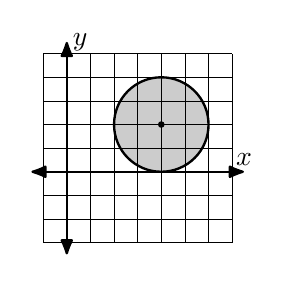
\begin{tikzpicture}[scale=0.3]

\fill [fill=\drawfill] (4,2) circle (2);

\draw [line width=0.1mm] (-1,-3) grid (7,5);
 
\draw[line width=0.3mm, <->, >={Latex[round]}] (-1.5, 0) -- (7.5, 0);

\draw[line width=0.3mm, <->, >={Latex[round]}] (0, -3.5) -- (0, 5.5);

\draw [black, line width=0.3mm] (4,2) circle (2);

\fill [fill=black] (4,2) circle (4pt);

\node[anchor=south, inner sep=2pt, rotate=0] (x-label) at (7.5,0) {$ x$};  

\node[anchor=west, inner sep=2pt, rotate=0] (y-label) at (0,5.5) {$ y$};  

\end{tikzpicture} 
%2
\item 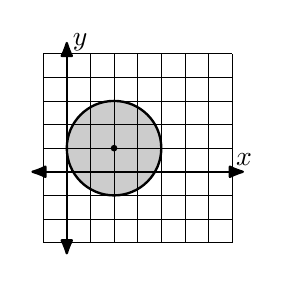
\begin{tikzpicture}[scale=0.3]

\fill [fill=\drawfill] (2,1) circle (2);

\draw [line width=0.1mm] (-1,-3) grid (7,5);
 
\draw[line width=0.3mm, <->, >={Latex[round]}] (-1.5, 0) -- (7.5, 0);

\draw[line width=0.3mm, <->, >={Latex[round]}] (0, -3.5) -- (0, 5.5);

\draw [black, line width=0.3mm] (2,1) circle (2);

\fill [fill=black] (2,1) circle (4pt);

\node[anchor=south, inner sep=2pt, rotate=0] (x-label) at (7.5,0) {$ x$};  

\node[anchor=west, inner sep=2pt, rotate=0] (y-label) at (0,5.5) {$ y$};  

\end{tikzpicture} 
%3
\item 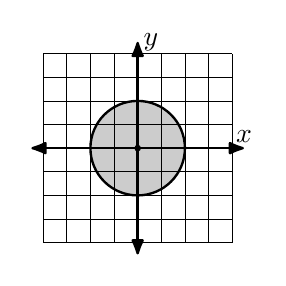
\begin{tikzpicture}[scale=0.3]

\fill [fill=\drawfill] (0,0) circle (2);

\draw [line width=0.1mm] (-4,-4) grid (4,4);
 
\draw[line width=0.3mm, <->, >={Latex[round]}] (-4.5, 0) -- (4.5, 0);

\draw[line width=0.3mm, <->, >={Latex[round]}] (0, -4.5) -- (0, 4.5);

\draw [black, line width=0.3mm] (0,0) circle (2);

\fill [fill=black] (0,0) circle (4pt);

\node[anchor=south, inner sep=2pt, rotate=0] (x-label) at (4.5,0) {$ x$};  

\node[anchor=west, inner sep=2pt, rotate=0] (y-label) at (0,4.5) {$ y$};  

\end{tikzpicture} 
%4
\item 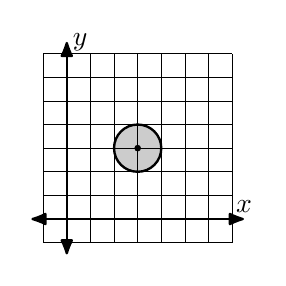
\begin{tikzpicture}[scale=0.3]

\fill [fill=\drawfill] (3,3) circle (1);

\draw [line width=0.1mm] (-1,-1) grid (7,7);
 
\draw[line width=0.3mm, <->, >={Latex[round]}] (-1.5, 0) -- (7.5, 0);

\draw[line width=0.3mm, <->, >={Latex[round]}] (0, -1.5) -- (0, 7.5);

\draw [black, line width=0.3mm] (3,3) circle (1);

\fill [fill=black] (3,3) circle (4pt);

\node[anchor=south, inner sep=2pt, rotate=0] (x-label) at (7.5,0) {$ x$};  

\node[anchor=west, inner sep=2pt, rotate=0] (y-label) at (0,7.5) {$ y$};  

\end{tikzpicture} 
%5 
\item 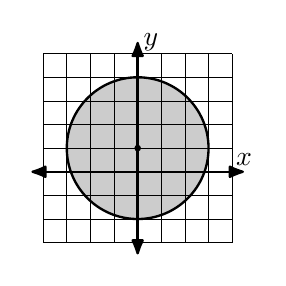
\begin{tikzpicture}[scale=0.3]

\fill [fill=\drawfill] (0,1) circle (3);

\draw [line width=0.1mm] (-4,-3) grid (4,5);
 
\draw[line width=0.3mm, <->, >={Latex[round]}] (-4.5, 0) -- (4.5, 0);

\draw[line width=0.3mm, <->, >={Latex[round]}] (0, -3.5) -- (0, 5.5);

\draw [black, line width=0.3mm] (0,1) circle (3);

\fill [fill=black] (0,1) circle (4pt);

\node[anchor=south, inner sep=2pt, rotate=0] (x-label) at (4.5,0) {$ x$};  

\node[anchor=west, inner sep=2pt, rotate=0] (y-label) at (0,5.5) {$ y$};  

\end{tikzpicture} 
%6
\item 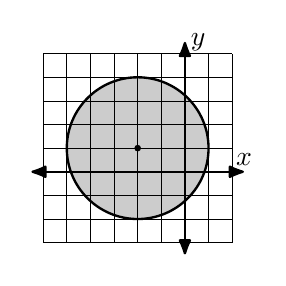
\begin{tikzpicture}[scale=0.3]

\fill [fill=\drawfill] (-2,1) circle (3);

\draw [line width=0.1mm] (-6,-3) grid (2,5);
 
\draw[line width=0.3mm, <->, >={Latex[round]}] (-6.5, 0) -- (2.5, 0);

\draw[line width=0.3mm, <->, >={Latex[round]}] (0, -3.5) -- (0, 5.5);

\draw [black, line width=0.3mm] (-2,1) circle (3);

\fill [fill=black] (-2,1) circle (4pt);

\node[anchor=south, inner sep=2pt, rotate=0] (x-label) at (2.5,0) {$ x$};  

\node[anchor=west, inner sep=2pt, rotate=0] (y-label) at (0,5.5) {$ y$};  

\end{tikzpicture} 
\end{multicols} 
\end{enumerate}  
%B
%\item \hspce 
%\begin{center}
\vspace*{1ex}
\scalebox{0.8}{
\noindent\begin{minipage}{\textwidth}
{

B. Find the center and radius of each circle with the given equation. 
\begin{enumerate}[label = \arabic*. ]
\begin{multicols}{2}

%1
\item \hspce $2x^2 + 2y^2 =32 $
%2
\item \hspce $x^2 + (y+5)^2 =100 $
%3
\item \hspce $(x-5)^2 + y^2 =169 $
%4
\item \hspce $(x+2)^2 + (y-4)^2 =36 $
%5 
%\item \hspce $(x-3)^2 + (y+2)^2 =16 $

\end{multicols} 
\end{enumerate}  
%C
%\item \hspce 
%end{enumerate}  
C. Write an equation of circle $C$ based on the given information. 
\begin{enumerate}[label = \arabic*. ]
%1
\item Center at (5, 4) and touching the x-axis 
%2
\item Center at (10, 4) and passing through (2, 2)
%3
\item Center at (3, 8) and passing through the origin 
%4
\item Center at (2, 5) and tangent to the y-axis
%5 
\item A circle with area 49 $\text{cm}^2 $ and center at (2, 5)
\end{enumerate}   

}
\end{minipage}}
%\end{center} 

%%D
%\item 
%\begin{center}
\vspace*{1ex}
\scalebox{0.75}{
\noindent\begin{minipage}{\textwidth}
{
D. Write each equation of a circle in general form. 
\begin{enumerate}[label = \arabic*. ]
\begin{multicols}{2}

%1
\item \hspce  $(x-2)^2 + (y-4)^2 = 36$
%2
\item \hspce  $(x+4)^2 + (y-9)^2 = 144$
%3
\item  \hspce $(x-6)^2 + (y-1)^2 = 81$
%4
%\item \hspce  $(x-8)^2 + (y+7)^2 = 225$
%5 
\item \hspce  $x^2 + (y-5)^2 = 36$
\end{multicols} 
\end{enumerate}  

%E
%\item 
E. Transform each equation to standard form, then give the coordinates of the center and the radius. 
\begin{enumerate}[label = \arabic*. ]
\begin{multicols}{2}
%1
\item  $x^2 + y^2 -2x -8y -47 =0$
%2
\item  $x^2 + y^2 +4x -4y -28 =0$
%3
\item  $x^2 + y^2 +10x +4y -3 =0$
%4
\item  $x^2 + y^2 +8y -84 =0$
%5 
%\item \hspce $x^2 + y^2 +8x -6y -39 =0$
\end{multicols} 
\end{enumerate}  
}
\end{minipage}}
%\end{center}  
\vspace*{1ex}
%\def\curdir{/storage/emulated/0/Documents/documents/latex/1920/Grade-10/3rd/equation-and-graph-of-a-circle/fb}

%\textbf{Practice Exercises}
\textbf{Problem Set}

\vspce

%\begin{enumerate}[label = \Alph*. ]
%A
%\item \hspce
A. Give the radius and coordinates of the center of the circle. Then write the equation in standard form. 
\begin{enumerate}[label = \arabic*. ]

\begin{multicols}{3}
%1 
\item 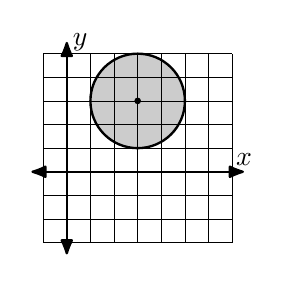
\begin{tikzpicture}[scale=0.3]

\filldraw [fill=\drawfill, line width=0.3mm] (3,3) circle (2);

\draw [line width=0.1mm] (-1,-3) grid (7,5);
 
\draw[line width=0.3mm, <->, >={Latex[round]}] (-1.5, 0) -- (7.5, 0);

\draw[line width=0.3mm, <->, >={Latex[round]}] (0, -3.5) -- (0, 5.5);

%\fill [opacity=.5,fill=\drawfill] (4,2) circle (2);

\fill [fill=black] (3,3) circle (4pt);

\node[anchor=south, inner sep=2pt, rotate=0] (x-label) at (7.5,0) {$ x$};  

\node[anchor=west, inner sep=2pt, rotate=0] (y-label) at (0,5.5) {$ y$};  

\end{tikzpicture} 
%2
\item 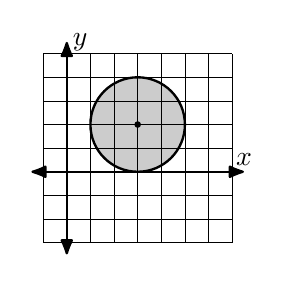
\begin{tikzpicture}[scale=0.3]

\filldraw [fill=\drawfill, line width=0.3mm] (3,2) circle (2);

\fill [fill=black] (3,2) circle (4pt);

\draw [line width=0.1mm] (-1,-3) grid (7,5);
 
\draw[line width=0.3mm, <->, >={Latex[round]}] (-1.5, 0) -- (7.5, 0);

\draw[line width=0.3mm, <->, >={Latex[round]}] (0, -3.5) -- (0, 5.5);

\node[anchor=south, inner sep=2pt, rotate=0] (x-label) at (7.5,0) {$ x$};  

\node[anchor=west, inner sep=2pt, rotate=0] (y-label) at (0,5.5) {$ y$};  

\end{tikzpicture} 
%3
\item 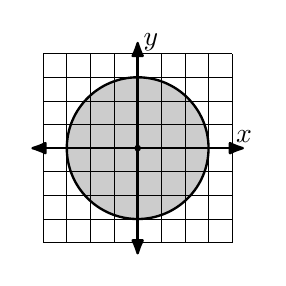
\begin{tikzpicture}[scale=0.3]

\filldraw [fill=\drawfill, line width=0.3mm] (0,0) circle (3);

\fill [fill=black] (0,0) circle (4pt);

\draw [line width=0.1mm] (-4,-4) grid (4,4);
 
\draw[line width=0.3mm, <->, >={Latex[round]}] (-4.5, 0) -- (4.5, 0);

\draw[line width=0.3mm, <->, >={Latex[round]}] (0, -4.5) -- (0, 4.5);

\node[anchor=south, inner sep=2pt, rotate=0] (x-label) at (4.5,0) {$ x$};  

\node[anchor=west, inner sep=2pt, rotate=0] (y-label) at (0,4.5) {$ y$};  

\end{tikzpicture} 
%4
\item 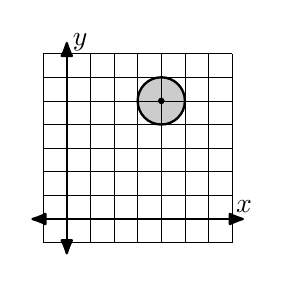
\begin{tikzpicture}[scale=0.3]

\filldraw [fill=\drawfill, line width=0.3mm] (4,5) circle (1);

\fill [fill=black] (4,5) circle (4pt);

\draw [line width=0.1mm] (-1,-1) grid (7,7);
 
\draw[line width=0.3mm, <->, >={Latex[round]}] (-1.5, 0) -- (7.5, 0);

\draw[line width=0.3mm, <->, >={Latex[round]}] (0, -1.5) -- (0, 7.5);

\node[anchor=south, inner sep=2pt, rotate=0] (x-label) at (7.5,0) {$ x$};  

\node[anchor=west, inner sep=2pt, rotate=0] (y-label) at (0,7.5) {$ y$};  

\end{tikzpicture} 
%5 
\item 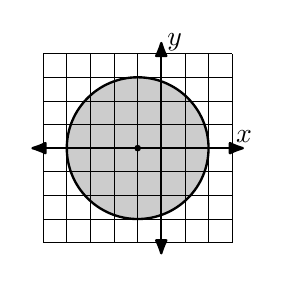
\begin{tikzpicture}[scale=0.3]

\filldraw [fill=\drawfill, line width=0.3mm] (-1,0) circle (3);

\fill [fill=black] (-1,0) circle (4pt);

\draw [line width=0.1mm] (-5,-4) grid (3,4);
 
\draw[line width=0.3mm, <->, >={Latex[round]}] (-5.5, 0) -- (3.5, 0);

\draw[line width=0.3mm, <->, >={Latex[round]}] (0, -4.5) -- (0, 4.5);

\node[anchor=south, inner sep=2pt, rotate=0] (x-label) at (3.5,0) {$ x$};  

\node[anchor=west, inner sep=2pt, rotate=0] (y-label) at (0,4.5) {$ y$};  

\end{tikzpicture} 
%6
\item 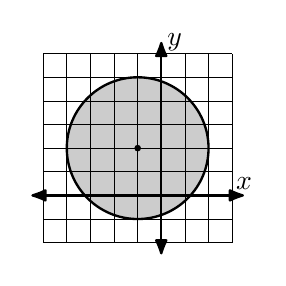
\begin{tikzpicture}[scale=0.3]

\filldraw [fill=\drawfill, line width=0.3mm] (-1,2) circle (3);

\fill [fill=black] (-1,2) circle (4pt);

\draw [line width=0.1mm] (-5,-2) grid (3,6);
 
\draw[line width=0.3mm, <->, >={Latex[round]}] (-5.5, 0) -- (3.5, 0);

\draw[line width=0.3mm, <->, >={Latex[round]}] (0, -2.5) -- (0, 6.5);

\node[anchor=south, inner sep=2pt, rotate=0] (x-label) at (3.5,0) {$ x$};  

\node[anchor=west, inner sep=2pt, rotate=0] (y-label) at (0,6.5) {$ y$};  


\end{tikzpicture} 
\end{multicols} 
\end{enumerate}  
%B
%\item \hspce 
%\begin{center}
%\vspace*{-2ex}
\scalebox{0.75}{
\noindent\begin{minipage}{\textwidth}
{
B. Find the center and radius of each circle with the given equation. 
\begin{enumerate}[label = \arabic*. ]
\begin{multicols}{2}
%1
\item \hspce $3x^2 + 3y^2 =12 $
%2
\item \hspce $x^2 + (y+4)^2 =81 $
%3
\item \hspce $(x-3)^2 + y^2 =144 $
%4
\item \hspce $(x+4)^2 + (y-3)^2 =64 $
%5 
%\item \hspce $(x-5)^2 + (y+1)^2 =49 $
\end{multicols} 
\end{enumerate}  
%C
%\item \hspce 
C. Write an equation of circle $C$ based on the given information. 
\begin{enumerate}[label = \arabic*. ]
%1
\item Center at (3, 2) and touching the x-axis 
%2
\item Center at (7, 5) and passing through (3, 4)
%3
\item Center at (4, 7) and passing through the origin 
%4
\item Center at (3, 7) and tangent to the y-axis
%5 
\item A circle with area 64 $\text{cm}^2 $ and center at (3, 6)
\end{enumerate}   

%D
%\item 
D. Write each equation of a circle in general form. 
\begin{enumerate}[label = \arabic*. ]
\begin{multicols}{2}
%1
\item \hspce  $(x-7)^2 + y^2 = 64$
%2
\item \hspce  $x^2 + (y+2)^2 = 49$
%3
\item  \hspce $(x+2)^2 + y^2 = 100$
%4
\item \hspce  $(x-5)^2 + (y-5)^2 = 27$
%5 
%\item \hspce  $(x+4)^2 + (y+4)^2 = 32$
\end{multicols} 
\end{enumerate}  

%E
%\item 
E. Transform each equation to standard form, then give the coordinates of the center and the radius. 
\begin{enumerate}[label = \arabic*. ]
\begin{multicols}{2}
%1
\item  $x^2 + y^2 -8x +2y -32 =0$
%2
\item   $x^2 + y^2 -6x -10y +18 =0$
%3
\item  $x^2 + y^2 - 6 x - 2 y - 15=0$
%4
\item  $x^2 + y^2 - 4 x + 6 y + 4 =0$
%5 
%\item \hspce $x^2 + y^2- 2 x  + 8 y - 47 =0$
\end{multicols} 
\end{enumerate}  

%\end{enumerate}  
}
\end{minipage}}
%\end{center}  

\end{frame}

\vertadjust
\begin{frame} %2
%\begin{center}
\textbf{The Equation of a Circle 
}
\end{center}

\vspce 
%\begin{center}
\vspace*{1ex}
\scalebox{0.8}{
\noindent\begin{minipage}{\textwidth}
{

\textbf{Standard Form}

The equation of a circle centered at the origin $(0, 0)$ and radius \textbf{r} is given by \[
x^2 + y^2 = r^2.
\]

\vspce 

The equation of a circle centered at $(h, k)$ having a radius of length \textbf{r} is  \[
(x-h)^2 + (y-k)^2 = r^2.
\] 

\vspce 
\textbf{General Form}

The general equation of a circle is \[x^2 + y^2 + Dx +Ey +F = 0,\] where $D$, $E$, and $F$ are real numbers, 
$D=-2h$, 
$E=-2k$, 
$F=h^2+k^2-r^2$. 
}
\end{minipage}}
  
%\def\curdir{/storage/emulated/0/Documents/documents/latex/1920/Grade-10/3rd/equation-and-graph-of-a-circle/fa}

\textbf{Practice Exercises}
%\textbf{Problem Set}

\vspce

%\begin{enumerate}[label = \Alph*. ]
%A
%\item \hspce 
A. Give the radius and coordinates of the center of the circle. Then write the equation in standard form. 
\begin{enumerate}[label = \arabic*. ]

\begin{multicols}{3}
%1 
\item 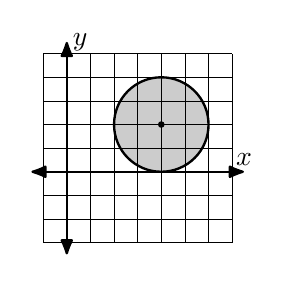
\begin{tikzpicture}[scale=0.3]

\fill [fill=\drawfill] (4,2) circle (2);

\draw [line width=0.1mm] (-1,-3) grid (7,5);
 
\draw[line width=0.3mm, <->, >={Latex[round]}] (-1.5, 0) -- (7.5, 0);

\draw[line width=0.3mm, <->, >={Latex[round]}] (0, -3.5) -- (0, 5.5);

\draw [black, line width=0.3mm] (4,2) circle (2);

\fill [fill=black] (4,2) circle (4pt);

\node[anchor=south, inner sep=2pt, rotate=0] (x-label) at (7.5,0) {$ x$};  

\node[anchor=west, inner sep=2pt, rotate=0] (y-label) at (0,5.5) {$ y$};  

\end{tikzpicture} 
%2
\item 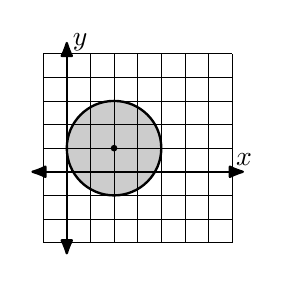
\begin{tikzpicture}[scale=0.3]

\fill [fill=\drawfill] (2,1) circle (2);

\draw [line width=0.1mm] (-1,-3) grid (7,5);
 
\draw[line width=0.3mm, <->, >={Latex[round]}] (-1.5, 0) -- (7.5, 0);

\draw[line width=0.3mm, <->, >={Latex[round]}] (0, -3.5) -- (0, 5.5);

\draw [black, line width=0.3mm] (2,1) circle (2);

\fill [fill=black] (2,1) circle (4pt);

\node[anchor=south, inner sep=2pt, rotate=0] (x-label) at (7.5,0) {$ x$};  

\node[anchor=west, inner sep=2pt, rotate=0] (y-label) at (0,5.5) {$ y$};  

\end{tikzpicture} 
%3
\item 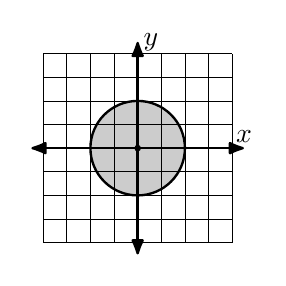
\begin{tikzpicture}[scale=0.3]

\fill [fill=\drawfill] (0,0) circle (2);

\draw [line width=0.1mm] (-4,-4) grid (4,4);
 
\draw[line width=0.3mm, <->, >={Latex[round]}] (-4.5, 0) -- (4.5, 0);

\draw[line width=0.3mm, <->, >={Latex[round]}] (0, -4.5) -- (0, 4.5);

\draw [black, line width=0.3mm] (0,0) circle (2);

\fill [fill=black] (0,0) circle (4pt);

\node[anchor=south, inner sep=2pt, rotate=0] (x-label) at (4.5,0) {$ x$};  

\node[anchor=west, inner sep=2pt, rotate=0] (y-label) at (0,4.5) {$ y$};  

\end{tikzpicture} 
%4
\item 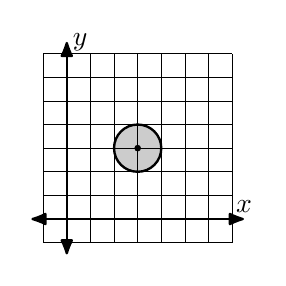
\begin{tikzpicture}[scale=0.3]

\fill [fill=\drawfill] (3,3) circle (1);

\draw [line width=0.1mm] (-1,-1) grid (7,7);
 
\draw[line width=0.3mm, <->, >={Latex[round]}] (-1.5, 0) -- (7.5, 0);

\draw[line width=0.3mm, <->, >={Latex[round]}] (0, -1.5) -- (0, 7.5);

\draw [black, line width=0.3mm] (3,3) circle (1);

\fill [fill=black] (3,3) circle (4pt);

\node[anchor=south, inner sep=2pt, rotate=0] (x-label) at (7.5,0) {$ x$};  

\node[anchor=west, inner sep=2pt, rotate=0] (y-label) at (0,7.5) {$ y$};  

\end{tikzpicture} 
%5 
\item 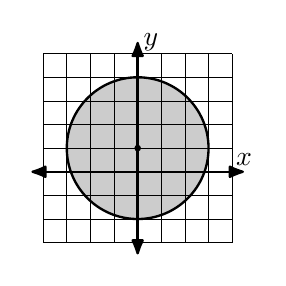
\begin{tikzpicture}[scale=0.3]

\fill [fill=\drawfill] (0,1) circle (3);

\draw [line width=0.1mm] (-4,-3) grid (4,5);
 
\draw[line width=0.3mm, <->, >={Latex[round]}] (-4.5, 0) -- (4.5, 0);

\draw[line width=0.3mm, <->, >={Latex[round]}] (0, -3.5) -- (0, 5.5);

\draw [black, line width=0.3mm] (0,1) circle (3);

\fill [fill=black] (0,1) circle (4pt);

\node[anchor=south, inner sep=2pt, rotate=0] (x-label) at (4.5,0) {$ x$};  

\node[anchor=west, inner sep=2pt, rotate=0] (y-label) at (0,5.5) {$ y$};  

\end{tikzpicture} 
%6
\item 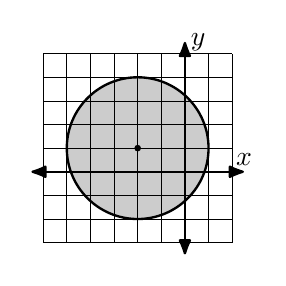
\begin{tikzpicture}[scale=0.3]

\fill [fill=\drawfill] (-2,1) circle (3);

\draw [line width=0.1mm] (-6,-3) grid (2,5);
 
\draw[line width=0.3mm, <->, >={Latex[round]}] (-6.5, 0) -- (2.5, 0);

\draw[line width=0.3mm, <->, >={Latex[round]}] (0, -3.5) -- (0, 5.5);

\draw [black, line width=0.3mm] (-2,1) circle (3);

\fill [fill=black] (-2,1) circle (4pt);

\node[anchor=south, inner sep=2pt, rotate=0] (x-label) at (2.5,0) {$ x$};  

\node[anchor=west, inner sep=2pt, rotate=0] (y-label) at (0,5.5) {$ y$};  

\end{tikzpicture} 
\end{multicols} 
\end{enumerate}  
%B
%\item \hspce 
%\begin{center}
\vspace*{1ex}
\scalebox{0.8}{
\noindent\begin{minipage}{\textwidth}
{

B. Find the center and radius of each circle with the given equation. 
\begin{enumerate}[label = \arabic*. ]
\begin{multicols}{2}

%1
\item \hspce $2x^2 + 2y^2 =32 $
%2
\item \hspce $x^2 + (y+5)^2 =100 $
%3
\item \hspce $(x-5)^2 + y^2 =169 $
%4
\item \hspce $(x+2)^2 + (y-4)^2 =36 $
%5 
%\item \hspce $(x-3)^2 + (y+2)^2 =16 $

\end{multicols} 
\end{enumerate}  
%C
%\item \hspce 
%end{enumerate}  
C. Write an equation of circle $C$ based on the given information. 
\begin{enumerate}[label = \arabic*. ]
%1
\item Center at (5, 4) and touching the x-axis 
%2
\item Center at (10, 4) and passing through (2, 2)
%3
\item Center at (3, 8) and passing through the origin 
%4
\item Center at (2, 5) and tangent to the y-axis
%5 
\item A circle with area 49 $\text{cm}^2 $ and center at (2, 5)
\end{enumerate}   

}
\end{minipage}}
%\end{center} 

%D
%\item 
%\begin{center}
\vspace*{1ex}
\scalebox{0.75}{
\noindent\begin{minipage}{\textwidth}
{
D. Write each equation of a circle in general form. 
\begin{enumerate}[label = \arabic*. ]
\begin{multicols}{2}

%1
\item \hspce  $(x-2)^2 + (y-4)^2 = 36$
%2
\item \hspce  $(x+4)^2 + (y-9)^2 = 144$
%3
\item  \hspce $(x-6)^2 + (y-1)^2 = 81$
%4
%\item \hspce  $(x-8)^2 + (y+7)^2 = 225$
%5 
\item \hspce  $x^2 + (y-5)^2 = 36$
\end{multicols} 
\end{enumerate}  

%E
%\item 
E. Transform each equation to standard form, then give the coordinates of the center and the radius. 
\begin{enumerate}[label = \arabic*. ]
\begin{multicols}{2}
%1
\item  $x^2 + y^2 -2x -8y -47 =0$
%2
\item  $x^2 + y^2 +4x -4y -28 =0$
%3
\item  $x^2 + y^2 +10x +4y -3 =0$
%4
\item  $x^2 + y^2 +8y -84 =0$
%5 
%\item \hspce $x^2 + y^2 +8x -6y -39 =0$
\end{multicols} 
\end{enumerate}  
}
\end{minipage}}
%\end{center}  
\vspace*{1ex}
\def\curdir{/storage/emulated/0/Documents/documents/latex/1920/Grade-10/3rd/equation-and-graph-of-a-circle/fb}

%\textbf{Practice Exercises}
\textbf{Problem Set}

\vspce

%\begin{enumerate}[label = \Alph*. ]
%A
%\item \hspce
A. Give the radius and coordinates of the center of the circle. Then write the equation in standard form. 
\begin{enumerate}[label = \arabic*. ]

\begin{multicols}{3}
%1 
\item 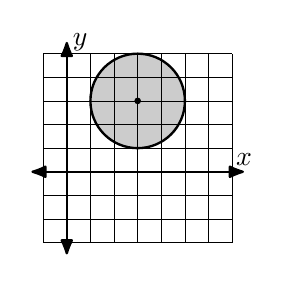
\begin{tikzpicture}[scale=0.3]

\filldraw [fill=\drawfill, line width=0.3mm] (3,3) circle (2);

\draw [line width=0.1mm] (-1,-3) grid (7,5);
 
\draw[line width=0.3mm, <->, >={Latex[round]}] (-1.5, 0) -- (7.5, 0);

\draw[line width=0.3mm, <->, >={Latex[round]}] (0, -3.5) -- (0, 5.5);

%\fill [opacity=.5,fill=\drawfill] (4,2) circle (2);

\fill [fill=black] (3,3) circle (4pt);

\node[anchor=south, inner sep=2pt, rotate=0] (x-label) at (7.5,0) {$ x$};  

\node[anchor=west, inner sep=2pt, rotate=0] (y-label) at (0,5.5) {$ y$};  

\end{tikzpicture} 
%2
\item 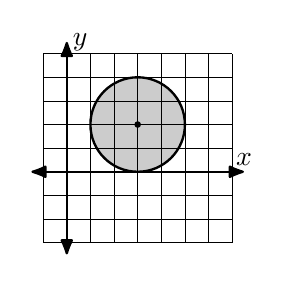
\begin{tikzpicture}[scale=0.3]

\filldraw [fill=\drawfill, line width=0.3mm] (3,2) circle (2);

\fill [fill=black] (3,2) circle (4pt);

\draw [line width=0.1mm] (-1,-3) grid (7,5);
 
\draw[line width=0.3mm, <->, >={Latex[round]}] (-1.5, 0) -- (7.5, 0);

\draw[line width=0.3mm, <->, >={Latex[round]}] (0, -3.5) -- (0, 5.5);

\node[anchor=south, inner sep=2pt, rotate=0] (x-label) at (7.5,0) {$ x$};  

\node[anchor=west, inner sep=2pt, rotate=0] (y-label) at (0,5.5) {$ y$};  

\end{tikzpicture} 
%3
\item 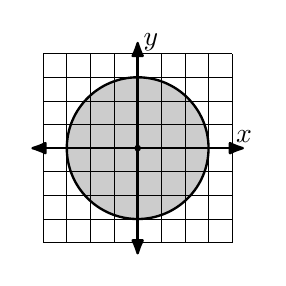
\begin{tikzpicture}[scale=0.3]

\filldraw [fill=\drawfill, line width=0.3mm] (0,0) circle (3);

\fill [fill=black] (0,0) circle (4pt);

\draw [line width=0.1mm] (-4,-4) grid (4,4);
 
\draw[line width=0.3mm, <->, >={Latex[round]}] (-4.5, 0) -- (4.5, 0);

\draw[line width=0.3mm, <->, >={Latex[round]}] (0, -4.5) -- (0, 4.5);

\node[anchor=south, inner sep=2pt, rotate=0] (x-label) at (4.5,0) {$ x$};  

\node[anchor=west, inner sep=2pt, rotate=0] (y-label) at (0,4.5) {$ y$};  

\end{tikzpicture} 
%4
\item 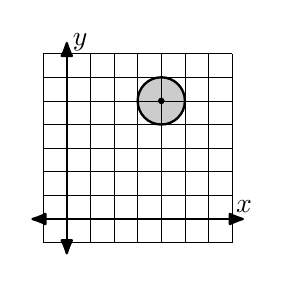
\begin{tikzpicture}[scale=0.3]

\filldraw [fill=\drawfill, line width=0.3mm] (4,5) circle (1);

\fill [fill=black] (4,5) circle (4pt);

\draw [line width=0.1mm] (-1,-1) grid (7,7);
 
\draw[line width=0.3mm, <->, >={Latex[round]}] (-1.5, 0) -- (7.5, 0);

\draw[line width=0.3mm, <->, >={Latex[round]}] (0, -1.5) -- (0, 7.5);

\node[anchor=south, inner sep=2pt, rotate=0] (x-label) at (7.5,0) {$ x$};  

\node[anchor=west, inner sep=2pt, rotate=0] (y-label) at (0,7.5) {$ y$};  

\end{tikzpicture} 
%5 
\item 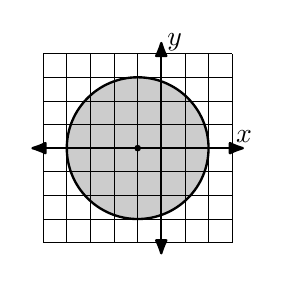
\begin{tikzpicture}[scale=0.3]

\filldraw [fill=\drawfill, line width=0.3mm] (-1,0) circle (3);

\fill [fill=black] (-1,0) circle (4pt);

\draw [line width=0.1mm] (-5,-4) grid (3,4);
 
\draw[line width=0.3mm, <->, >={Latex[round]}] (-5.5, 0) -- (3.5, 0);

\draw[line width=0.3mm, <->, >={Latex[round]}] (0, -4.5) -- (0, 4.5);

\node[anchor=south, inner sep=2pt, rotate=0] (x-label) at (3.5,0) {$ x$};  

\node[anchor=west, inner sep=2pt, rotate=0] (y-label) at (0,4.5) {$ y$};  

\end{tikzpicture} 
%6
\item 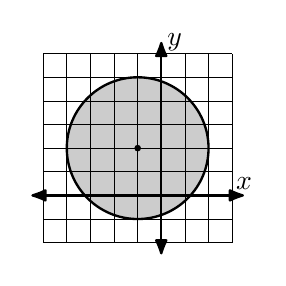
\begin{tikzpicture}[scale=0.3]

\filldraw [fill=\drawfill, line width=0.3mm] (-1,2) circle (3);

\fill [fill=black] (-1,2) circle (4pt);

\draw [line width=0.1mm] (-5,-2) grid (3,6);
 
\draw[line width=0.3mm, <->, >={Latex[round]}] (-5.5, 0) -- (3.5, 0);

\draw[line width=0.3mm, <->, >={Latex[round]}] (0, -2.5) -- (0, 6.5);

\node[anchor=south, inner sep=2pt, rotate=0] (x-label) at (3.5,0) {$ x$};  

\node[anchor=west, inner sep=2pt, rotate=0] (y-label) at (0,6.5) {$ y$};  


\end{tikzpicture} 
\end{multicols} 
\end{enumerate}  
%B
%\item \hspce 
%\begin{center}
%\vspace*{-2ex}
\scalebox{0.75}{
\noindent\begin{minipage}{\textwidth}
{
B. Find the center and radius of each circle with the given equation. 
\begin{enumerate}[label = \arabic*. ]
\begin{multicols}{2}
%1
\item \hspce $3x^2 + 3y^2 =12 $
%2
\item \hspce $x^2 + (y+4)^2 =81 $
%3
\item \hspce $(x-3)^2 + y^2 =144 $
%4
\item \hspce $(x+4)^2 + (y-3)^2 =64 $
%5 
%\item \hspce $(x-5)^2 + (y+1)^2 =49 $
\end{multicols} 
\end{enumerate}  
%C
%\item \hspce 
C. Write an equation of circle $C$ based on the given information. 
\begin{enumerate}[label = \arabic*. ]
%1
\item Center at (3, 2) and touching the x-axis 
%2
\item Center at (7, 5) and passing through (3, 4)
%3
\item Center at (4, 7) and passing through the origin 
%4
\item Center at (3, 7) and tangent to the y-axis
%5 
\item A circle with area 64 $\text{cm}^2 $ and center at (3, 6)
\end{enumerate}   

%D
%\item 
D. Write each equation of a circle in general form. 
\begin{enumerate}[label = \arabic*. ]
\begin{multicols}{2}
%1
\item \hspce  $(x-7)^2 + y^2 = 64$
%2
\item \hspce  $x^2 + (y+2)^2 = 49$
%3
\item  \hspce $(x+2)^2 + y^2 = 100$
%4
\item \hspce  $(x-5)^2 + (y-5)^2 = 27$
%5 
%\item \hspce  $(x+4)^2 + (y+4)^2 = 32$
\end{multicols} 
\end{enumerate}  

%E
%\item 
E. Transform each equation to standard form, then give the coordinates of the center and the radius. 
\begin{enumerate}[label = \arabic*. ]
\begin{multicols}{2}
%1
\item  $x^2 + y^2 -8x +2y -32 =0$
%2
\item   $x^2 + y^2 -6x -10y +18 =0$
%3
\item  $x^2 + y^2 - 6 x - 2 y - 15=0$
%4
\item  $x^2 + y^2 - 4 x + 6 y + 4 =0$
%5 
%\item \hspce $x^2 + y^2- 2 x  + 8 y - 47 =0$
\end{multicols} 
\end{enumerate}  

%\end{enumerate}  
}
\end{minipage}}
%\end{center}  

\end{frame}

%\vspace*{-2.7in} %legalpaper
\vertadjust
\begin{frame} %3
\begin{center}
\textbf{The Equation of a Circle 
}
\end{center}

\vspce 
%\begin{center}
\vspace*{1ex}
\scalebox{0.8}{
\noindent\begin{minipage}{\textwidth}
{

\textbf{Standard Form}

The equation of a circle centered at the origin $(0, 0)$ and radius \textbf{r} is given by \[
x^2 + y^2 = r^2.
\]

\vspce 

The equation of a circle centered at $(h, k)$ having a radius of length \textbf{r} is  \[
(x-h)^2 + (y-k)^2 = r^2.
\] 

\vspce 
\textbf{General Form}

The general equation of a circle is \[x^2 + y^2 + Dx +Ey +F = 0,\] where $D$, $E$, and $F$ are real numbers, 
$D=-2h$, 
$E=-2k$, 
$F=h^2+k^2-r^2$. 
}
\end{minipage}}
  
\def\curdir{/storage/emulated/0/Documents/documents/latex/1920/Grade-10/3rd/equation-and-graph-of-a-circle/fa}

\textbf{Practice Exercises}
%\textbf{Problem Set}

\vspce

%\begin{enumerate}[label = \Alph*. ]
%A
%\item \hspce 
A. Give the radius and coordinates of the center of the circle. Then write the equation in standard form. 
\begin{enumerate}[label = \arabic*. ]

\begin{multicols}{3}
%1 
\item 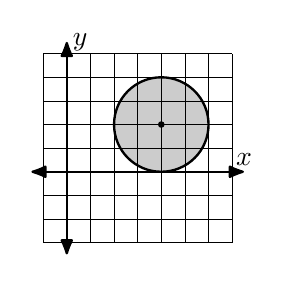
\begin{tikzpicture}[scale=0.3]

\fill [fill=\drawfill] (4,2) circle (2);

\draw [line width=0.1mm] (-1,-3) grid (7,5);
 
\draw[line width=0.3mm, <->, >={Latex[round]}] (-1.5, 0) -- (7.5, 0);

\draw[line width=0.3mm, <->, >={Latex[round]}] (0, -3.5) -- (0, 5.5);

\draw [black, line width=0.3mm] (4,2) circle (2);

\fill [fill=black] (4,2) circle (4pt);

\node[anchor=south, inner sep=2pt, rotate=0] (x-label) at (7.5,0) {$ x$};  

\node[anchor=west, inner sep=2pt, rotate=0] (y-label) at (0,5.5) {$ y$};  

\end{tikzpicture} 
%2
\item 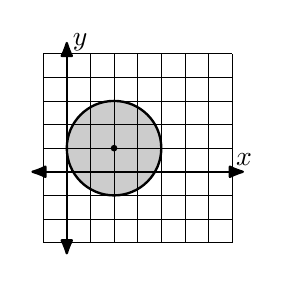
\begin{tikzpicture}[scale=0.3]

\fill [fill=\drawfill] (2,1) circle (2);

\draw [line width=0.1mm] (-1,-3) grid (7,5);
 
\draw[line width=0.3mm, <->, >={Latex[round]}] (-1.5, 0) -- (7.5, 0);

\draw[line width=0.3mm, <->, >={Latex[round]}] (0, -3.5) -- (0, 5.5);

\draw [black, line width=0.3mm] (2,1) circle (2);

\fill [fill=black] (2,1) circle (4pt);

\node[anchor=south, inner sep=2pt, rotate=0] (x-label) at (7.5,0) {$ x$};  

\node[anchor=west, inner sep=2pt, rotate=0] (y-label) at (0,5.5) {$ y$};  

\end{tikzpicture} 
%3
\item 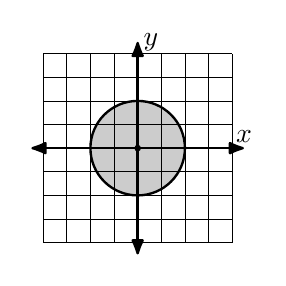
\begin{tikzpicture}[scale=0.3]

\fill [fill=\drawfill] (0,0) circle (2);

\draw [line width=0.1mm] (-4,-4) grid (4,4);
 
\draw[line width=0.3mm, <->, >={Latex[round]}] (-4.5, 0) -- (4.5, 0);

\draw[line width=0.3mm, <->, >={Latex[round]}] (0, -4.5) -- (0, 4.5);

\draw [black, line width=0.3mm] (0,0) circle (2);

\fill [fill=black] (0,0) circle (4pt);

\node[anchor=south, inner sep=2pt, rotate=0] (x-label) at (4.5,0) {$ x$};  

\node[anchor=west, inner sep=2pt, rotate=0] (y-label) at (0,4.5) {$ y$};  

\end{tikzpicture} 
%4
\item 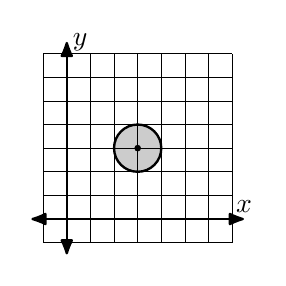
\begin{tikzpicture}[scale=0.3]

\fill [fill=\drawfill] (3,3) circle (1);

\draw [line width=0.1mm] (-1,-1) grid (7,7);
 
\draw[line width=0.3mm, <->, >={Latex[round]}] (-1.5, 0) -- (7.5, 0);

\draw[line width=0.3mm, <->, >={Latex[round]}] (0, -1.5) -- (0, 7.5);

\draw [black, line width=0.3mm] (3,3) circle (1);

\fill [fill=black] (3,3) circle (4pt);

\node[anchor=south, inner sep=2pt, rotate=0] (x-label) at (7.5,0) {$ x$};  

\node[anchor=west, inner sep=2pt, rotate=0] (y-label) at (0,7.5) {$ y$};  

\end{tikzpicture} 
%5 
\item 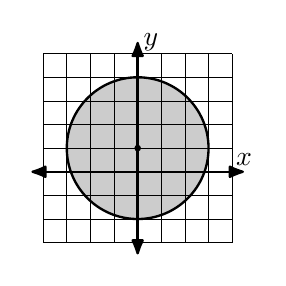
\begin{tikzpicture}[scale=0.3]

\fill [fill=\drawfill] (0,1) circle (3);

\draw [line width=0.1mm] (-4,-3) grid (4,5);
 
\draw[line width=0.3mm, <->, >={Latex[round]}] (-4.5, 0) -- (4.5, 0);

\draw[line width=0.3mm, <->, >={Latex[round]}] (0, -3.5) -- (0, 5.5);

\draw [black, line width=0.3mm] (0,1) circle (3);

\fill [fill=black] (0,1) circle (4pt);

\node[anchor=south, inner sep=2pt, rotate=0] (x-label) at (4.5,0) {$ x$};  

\node[anchor=west, inner sep=2pt, rotate=0] (y-label) at (0,5.5) {$ y$};  

\end{tikzpicture} 
%6
\item 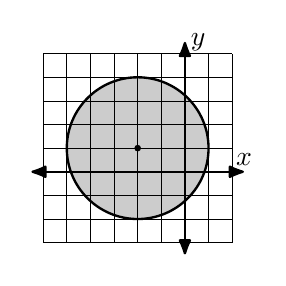
\begin{tikzpicture}[scale=0.3]

\fill [fill=\drawfill] (-2,1) circle (3);

\draw [line width=0.1mm] (-6,-3) grid (2,5);
 
\draw[line width=0.3mm, <->, >={Latex[round]}] (-6.5, 0) -- (2.5, 0);

\draw[line width=0.3mm, <->, >={Latex[round]}] (0, -3.5) -- (0, 5.5);

\draw [black, line width=0.3mm] (-2,1) circle (3);

\fill [fill=black] (-2,1) circle (4pt);

\node[anchor=south, inner sep=2pt, rotate=0] (x-label) at (2.5,0) {$ x$};  

\node[anchor=west, inner sep=2pt, rotate=0] (y-label) at (0,5.5) {$ y$};  

\end{tikzpicture} 
\end{multicols} 
\end{enumerate}  
%B
%\item \hspce 
%\begin{center}
\vspace*{1ex}
\scalebox{0.8}{
\noindent\begin{minipage}{\textwidth}
{

B. Find the center and radius of each circle with the given equation. 
\begin{enumerate}[label = \arabic*. ]
\begin{multicols}{2}

%1
\item \hspce $2x^2 + 2y^2 =32 $
%2
\item \hspce $x^2 + (y+5)^2 =100 $
%3
\item \hspce $(x-5)^2 + y^2 =169 $
%4
\item \hspce $(x+2)^2 + (y-4)^2 =36 $
%5 
%\item \hspce $(x-3)^2 + (y+2)^2 =16 $

\end{multicols} 
\end{enumerate}  
%C
%\item \hspce 
%end{enumerate}  
C. Write an equation of circle $C$ based on the given information. 
\begin{enumerate}[label = \arabic*. ]
%1
\item Center at (5, 4) and touching the x-axis 
%2
\item Center at (10, 4) and passing through (2, 2)
%3
\item Center at (3, 8) and passing through the origin 
%4
\item Center at (2, 5) and tangent to the y-axis
%5 
\item A circle with area 49 $\text{cm}^2 $ and center at (2, 5)
\end{enumerate}   

}
\end{minipage}}
%\end{center} 

%%D
%\item 
%\begin{center}
\vspace*{1ex}
\scalebox{0.75}{
\noindent\begin{minipage}{\textwidth}
{
D. Write each equation of a circle in general form. 
\begin{enumerate}[label = \arabic*. ]
\begin{multicols}{2}

%1
\item \hspce  $(x-2)^2 + (y-4)^2 = 36$
%2
\item \hspce  $(x+4)^2 + (y-9)^2 = 144$
%3
\item  \hspce $(x-6)^2 + (y-1)^2 = 81$
%4
%\item \hspce  $(x-8)^2 + (y+7)^2 = 225$
%5 
\item \hspce  $x^2 + (y-5)^2 = 36$
\end{multicols} 
\end{enumerate}  

%E
%\item 
E. Transform each equation to standard form, then give the coordinates of the center and the radius. 
\begin{enumerate}[label = \arabic*. ]
\begin{multicols}{2}
%1
\item  $x^2 + y^2 -2x -8y -47 =0$
%2
\item  $x^2 + y^2 +4x -4y -28 =0$
%3
\item  $x^2 + y^2 +10x +4y -3 =0$
%4
\item  $x^2 + y^2 +8y -84 =0$
%5 
%\item \hspce $x^2 + y^2 +8x -6y -39 =0$
\end{multicols} 
\end{enumerate}  
}
\end{minipage}}
%\end{center}  
\vspace*{1ex}
%\def\curdir{/storage/emulated/0/Documents/documents/latex/1920/Grade-10/3rd/equation-and-graph-of-a-circle/fb}

%\textbf{Practice Exercises}
\textbf{Problem Set}

\vspce

%\begin{enumerate}[label = \Alph*. ]
%A
%\item \hspce
A. Give the radius and coordinates of the center of the circle. Then write the equation in standard form. 
\begin{enumerate}[label = \arabic*. ]

\begin{multicols}{3}
%1 
\item 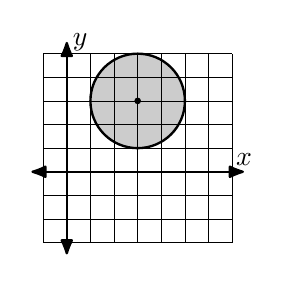
\begin{tikzpicture}[scale=0.3]

\filldraw [fill=\drawfill, line width=0.3mm] (3,3) circle (2);

\draw [line width=0.1mm] (-1,-3) grid (7,5);
 
\draw[line width=0.3mm, <->, >={Latex[round]}] (-1.5, 0) -- (7.5, 0);

\draw[line width=0.3mm, <->, >={Latex[round]}] (0, -3.5) -- (0, 5.5);

%\fill [opacity=.5,fill=\drawfill] (4,2) circle (2);

\fill [fill=black] (3,3) circle (4pt);

\node[anchor=south, inner sep=2pt, rotate=0] (x-label) at (7.5,0) {$ x$};  

\node[anchor=west, inner sep=2pt, rotate=0] (y-label) at (0,5.5) {$ y$};  

\end{tikzpicture} 
%2
\item 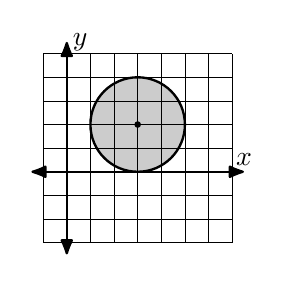
\begin{tikzpicture}[scale=0.3]

\filldraw [fill=\drawfill, line width=0.3mm] (3,2) circle (2);

\fill [fill=black] (3,2) circle (4pt);

\draw [line width=0.1mm] (-1,-3) grid (7,5);
 
\draw[line width=0.3mm, <->, >={Latex[round]}] (-1.5, 0) -- (7.5, 0);

\draw[line width=0.3mm, <->, >={Latex[round]}] (0, -3.5) -- (0, 5.5);

\node[anchor=south, inner sep=2pt, rotate=0] (x-label) at (7.5,0) {$ x$};  

\node[anchor=west, inner sep=2pt, rotate=0] (y-label) at (0,5.5) {$ y$};  

\end{tikzpicture} 
%3
\item 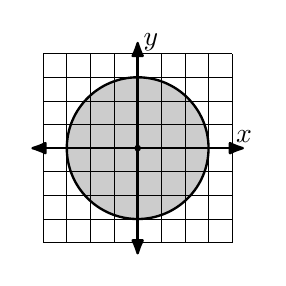
\begin{tikzpicture}[scale=0.3]

\filldraw [fill=\drawfill, line width=0.3mm] (0,0) circle (3);

\fill [fill=black] (0,0) circle (4pt);

\draw [line width=0.1mm] (-4,-4) grid (4,4);
 
\draw[line width=0.3mm, <->, >={Latex[round]}] (-4.5, 0) -- (4.5, 0);

\draw[line width=0.3mm, <->, >={Latex[round]}] (0, -4.5) -- (0, 4.5);

\node[anchor=south, inner sep=2pt, rotate=0] (x-label) at (4.5,0) {$ x$};  

\node[anchor=west, inner sep=2pt, rotate=0] (y-label) at (0,4.5) {$ y$};  

\end{tikzpicture} 
%4
\item 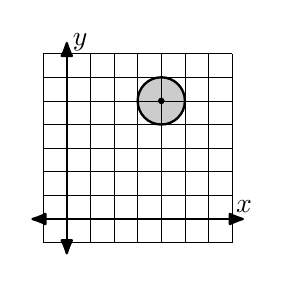
\begin{tikzpicture}[scale=0.3]

\filldraw [fill=\drawfill, line width=0.3mm] (4,5) circle (1);

\fill [fill=black] (4,5) circle (4pt);

\draw [line width=0.1mm] (-1,-1) grid (7,7);
 
\draw[line width=0.3mm, <->, >={Latex[round]}] (-1.5, 0) -- (7.5, 0);

\draw[line width=0.3mm, <->, >={Latex[round]}] (0, -1.5) -- (0, 7.5);

\node[anchor=south, inner sep=2pt, rotate=0] (x-label) at (7.5,0) {$ x$};  

\node[anchor=west, inner sep=2pt, rotate=0] (y-label) at (0,7.5) {$ y$};  

\end{tikzpicture} 
%5 
\item 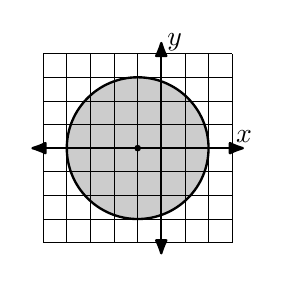
\begin{tikzpicture}[scale=0.3]

\filldraw [fill=\drawfill, line width=0.3mm] (-1,0) circle (3);

\fill [fill=black] (-1,0) circle (4pt);

\draw [line width=0.1mm] (-5,-4) grid (3,4);
 
\draw[line width=0.3mm, <->, >={Latex[round]}] (-5.5, 0) -- (3.5, 0);

\draw[line width=0.3mm, <->, >={Latex[round]}] (0, -4.5) -- (0, 4.5);

\node[anchor=south, inner sep=2pt, rotate=0] (x-label) at (3.5,0) {$ x$};  

\node[anchor=west, inner sep=2pt, rotate=0] (y-label) at (0,4.5) {$ y$};  

\end{tikzpicture} 
%6
\item 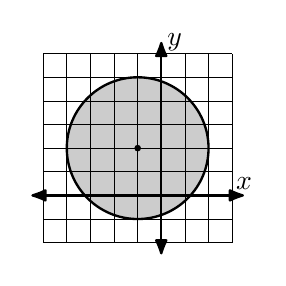
\begin{tikzpicture}[scale=0.3]

\filldraw [fill=\drawfill, line width=0.3mm] (-1,2) circle (3);

\fill [fill=black] (-1,2) circle (4pt);

\draw [line width=0.1mm] (-5,-2) grid (3,6);
 
\draw[line width=0.3mm, <->, >={Latex[round]}] (-5.5, 0) -- (3.5, 0);

\draw[line width=0.3mm, <->, >={Latex[round]}] (0, -2.5) -- (0, 6.5);

\node[anchor=south, inner sep=2pt, rotate=0] (x-label) at (3.5,0) {$ x$};  

\node[anchor=west, inner sep=2pt, rotate=0] (y-label) at (0,6.5) {$ y$};  


\end{tikzpicture} 
\end{multicols} 
\end{enumerate}  
%B
%\item \hspce 
%\begin{center}
%\vspace*{-2ex}
\scalebox{0.75}{
\noindent\begin{minipage}{\textwidth}
{
B. Find the center and radius of each circle with the given equation. 
\begin{enumerate}[label = \arabic*. ]
\begin{multicols}{2}
%1
\item \hspce $3x^2 + 3y^2 =12 $
%2
\item \hspce $x^2 + (y+4)^2 =81 $
%3
\item \hspce $(x-3)^2 + y^2 =144 $
%4
\item \hspce $(x+4)^2 + (y-3)^2 =64 $
%5 
%\item \hspce $(x-5)^2 + (y+1)^2 =49 $
\end{multicols} 
\end{enumerate}  
%C
%\item \hspce 
C. Write an equation of circle $C$ based on the given information. 
\begin{enumerate}[label = \arabic*. ]
%1
\item Center at (3, 2) and touching the x-axis 
%2
\item Center at (7, 5) and passing through (3, 4)
%3
\item Center at (4, 7) and passing through the origin 
%4
\item Center at (3, 7) and tangent to the y-axis
%5 
\item A circle with area 64 $\text{cm}^2 $ and center at (3, 6)
\end{enumerate}   

%D
%\item 
D. Write each equation of a circle in general form. 
\begin{enumerate}[label = \arabic*. ]
\begin{multicols}{2}
%1
\item \hspce  $(x-7)^2 + y^2 = 64$
%2
\item \hspce  $x^2 + (y+2)^2 = 49$
%3
\item  \hspce $(x+2)^2 + y^2 = 100$
%4
\item \hspce  $(x-5)^2 + (y-5)^2 = 27$
%5 
%\item \hspce  $(x+4)^2 + (y+4)^2 = 32$
\end{multicols} 
\end{enumerate}  

%E
%\item 
E. Transform each equation to standard form, then give the coordinates of the center and the radius. 
\begin{enumerate}[label = \arabic*. ]
\begin{multicols}{2}
%1
\item  $x^2 + y^2 -8x +2y -32 =0$
%2
\item   $x^2 + y^2 -6x -10y +18 =0$
%3
\item  $x^2 + y^2 - 6 x - 2 y - 15=0$
%4
\item  $x^2 + y^2 - 4 x + 6 y + 4 =0$
%5 
%\item \hspce $x^2 + y^2- 2 x  + 8 y - 47 =0$
\end{multicols} 
\end{enumerate}  

%\end{enumerate}  
}
\end{minipage}}
%\end{center}  

\end{frame}

%\vspace*{-2.7in} %legalpaper
\vertadjust
\begin{frame} %4
%\begin{center}
\textbf{The Equation of a Circle 
}
\end{center}

\vspce 
%\begin{center}
\vspace*{1ex}
\scalebox{0.8}{
\noindent\begin{minipage}{\textwidth}
{

\textbf{Standard Form}

The equation of a circle centered at the origin $(0, 0)$ and radius \textbf{r} is given by \[
x^2 + y^2 = r^2.
\]

\vspce 

The equation of a circle centered at $(h, k)$ having a radius of length \textbf{r} is  \[
(x-h)^2 + (y-k)^2 = r^2.
\] 

\vspce 
\textbf{General Form}

The general equation of a circle is \[x^2 + y^2 + Dx +Ey +F = 0,\] where $D$, $E$, and $F$ are real numbers, 
$D=-2h$, 
$E=-2k$, 
$F=h^2+k^2-r^2$. 
}
\end{minipage}}
  
%\def\curdir{/storage/emulated/0/Documents/documents/latex/1920/Grade-10/3rd/equation-and-graph-of-a-circle/fa}

\textbf{Practice Exercises}
%\textbf{Problem Set}

\vspce

%\begin{enumerate}[label = \Alph*. ]
%A
%\item \hspce 
A. Give the radius and coordinates of the center of the circle. Then write the equation in standard form. 
\begin{enumerate}[label = \arabic*. ]

\begin{multicols}{3}
%1 
\item 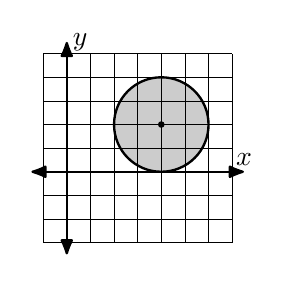
\begin{tikzpicture}[scale=0.3]

\fill [fill=\drawfill] (4,2) circle (2);

\draw [line width=0.1mm] (-1,-3) grid (7,5);
 
\draw[line width=0.3mm, <->, >={Latex[round]}] (-1.5, 0) -- (7.5, 0);

\draw[line width=0.3mm, <->, >={Latex[round]}] (0, -3.5) -- (0, 5.5);

\draw [black, line width=0.3mm] (4,2) circle (2);

\fill [fill=black] (4,2) circle (4pt);

\node[anchor=south, inner sep=2pt, rotate=0] (x-label) at (7.5,0) {$ x$};  

\node[anchor=west, inner sep=2pt, rotate=0] (y-label) at (0,5.5) {$ y$};  

\end{tikzpicture} 
%2
\item 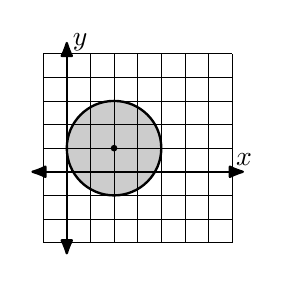
\begin{tikzpicture}[scale=0.3]

\fill [fill=\drawfill] (2,1) circle (2);

\draw [line width=0.1mm] (-1,-3) grid (7,5);
 
\draw[line width=0.3mm, <->, >={Latex[round]}] (-1.5, 0) -- (7.5, 0);

\draw[line width=0.3mm, <->, >={Latex[round]}] (0, -3.5) -- (0, 5.5);

\draw [black, line width=0.3mm] (2,1) circle (2);

\fill [fill=black] (2,1) circle (4pt);

\node[anchor=south, inner sep=2pt, rotate=0] (x-label) at (7.5,0) {$ x$};  

\node[anchor=west, inner sep=2pt, rotate=0] (y-label) at (0,5.5) {$ y$};  

\end{tikzpicture} 
%3
\item 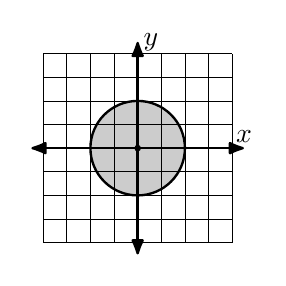
\begin{tikzpicture}[scale=0.3]

\fill [fill=\drawfill] (0,0) circle (2);

\draw [line width=0.1mm] (-4,-4) grid (4,4);
 
\draw[line width=0.3mm, <->, >={Latex[round]}] (-4.5, 0) -- (4.5, 0);

\draw[line width=0.3mm, <->, >={Latex[round]}] (0, -4.5) -- (0, 4.5);

\draw [black, line width=0.3mm] (0,0) circle (2);

\fill [fill=black] (0,0) circle (4pt);

\node[anchor=south, inner sep=2pt, rotate=0] (x-label) at (4.5,0) {$ x$};  

\node[anchor=west, inner sep=2pt, rotate=0] (y-label) at (0,4.5) {$ y$};  

\end{tikzpicture} 
%4
\item 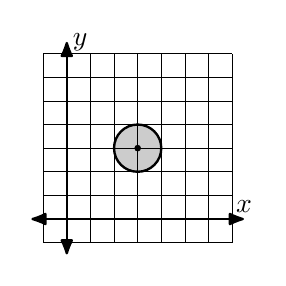
\begin{tikzpicture}[scale=0.3]

\fill [fill=\drawfill] (3,3) circle (1);

\draw [line width=0.1mm] (-1,-1) grid (7,7);
 
\draw[line width=0.3mm, <->, >={Latex[round]}] (-1.5, 0) -- (7.5, 0);

\draw[line width=0.3mm, <->, >={Latex[round]}] (0, -1.5) -- (0, 7.5);

\draw [black, line width=0.3mm] (3,3) circle (1);

\fill [fill=black] (3,3) circle (4pt);

\node[anchor=south, inner sep=2pt, rotate=0] (x-label) at (7.5,0) {$ x$};  

\node[anchor=west, inner sep=2pt, rotate=0] (y-label) at (0,7.5) {$ y$};  

\end{tikzpicture} 
%5 
\item 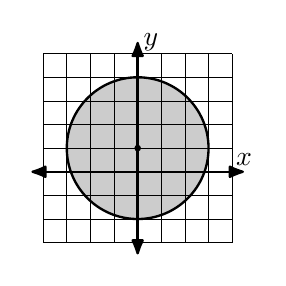
\begin{tikzpicture}[scale=0.3]

\fill [fill=\drawfill] (0,1) circle (3);

\draw [line width=0.1mm] (-4,-3) grid (4,5);
 
\draw[line width=0.3mm, <->, >={Latex[round]}] (-4.5, 0) -- (4.5, 0);

\draw[line width=0.3mm, <->, >={Latex[round]}] (0, -3.5) -- (0, 5.5);

\draw [black, line width=0.3mm] (0,1) circle (3);

\fill [fill=black] (0,1) circle (4pt);

\node[anchor=south, inner sep=2pt, rotate=0] (x-label) at (4.5,0) {$ x$};  

\node[anchor=west, inner sep=2pt, rotate=0] (y-label) at (0,5.5) {$ y$};  

\end{tikzpicture} 
%6
\item 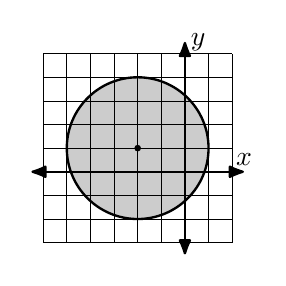
\begin{tikzpicture}[scale=0.3]

\fill [fill=\drawfill] (-2,1) circle (3);

\draw [line width=0.1mm] (-6,-3) grid (2,5);
 
\draw[line width=0.3mm, <->, >={Latex[round]}] (-6.5, 0) -- (2.5, 0);

\draw[line width=0.3mm, <->, >={Latex[round]}] (0, -3.5) -- (0, 5.5);

\draw [black, line width=0.3mm] (-2,1) circle (3);

\fill [fill=black] (-2,1) circle (4pt);

\node[anchor=south, inner sep=2pt, rotate=0] (x-label) at (2.5,0) {$ x$};  

\node[anchor=west, inner sep=2pt, rotate=0] (y-label) at (0,5.5) {$ y$};  

\end{tikzpicture} 
\end{multicols} 
\end{enumerate}  
%B
%\item \hspce 
%\begin{center}
\vspace*{1ex}
\scalebox{0.8}{
\noindent\begin{minipage}{\textwidth}
{

B. Find the center and radius of each circle with the given equation. 
\begin{enumerate}[label = \arabic*. ]
\begin{multicols}{2}

%1
\item \hspce $2x^2 + 2y^2 =32 $
%2
\item \hspce $x^2 + (y+5)^2 =100 $
%3
\item \hspce $(x-5)^2 + y^2 =169 $
%4
\item \hspce $(x+2)^2 + (y-4)^2 =36 $
%5 
%\item \hspce $(x-3)^2 + (y+2)^2 =16 $

\end{multicols} 
\end{enumerate}  
%C
%\item \hspce 
%end{enumerate}  
C. Write an equation of circle $C$ based on the given information. 
\begin{enumerate}[label = \arabic*. ]
%1
\item Center at (5, 4) and touching the x-axis 
%2
\item Center at (10, 4) and passing through (2, 2)
%3
\item Center at (3, 8) and passing through the origin 
%4
\item Center at (2, 5) and tangent to the y-axis
%5 
\item A circle with area 49 $\text{cm}^2 $ and center at (2, 5)
\end{enumerate}   

}
\end{minipage}}
%\end{center} 

%D
%\item 
%\begin{center}
\vspace*{1ex}
\scalebox{0.75}{
\noindent\begin{minipage}{\textwidth}
{
D. Write each equation of a circle in general form. 
\begin{enumerate}[label = \arabic*. ]
\begin{multicols}{2}

%1
\item \hspce  $(x-2)^2 + (y-4)^2 = 36$
%2
\item \hspce  $(x+4)^2 + (y-9)^2 = 144$
%3
\item  \hspce $(x-6)^2 + (y-1)^2 = 81$
%4
%\item \hspce  $(x-8)^2 + (y+7)^2 = 225$
%5 
\item \hspce  $x^2 + (y-5)^2 = 36$
\end{multicols} 
\end{enumerate}  

%E
%\item 
E. Transform each equation to standard form, then give the coordinates of the center and the radius. 
\begin{enumerate}[label = \arabic*. ]
\begin{multicols}{2}
%1
\item  $x^2 + y^2 -2x -8y -47 =0$
%2
\item  $x^2 + y^2 +4x -4y -28 =0$
%3
\item  $x^2 + y^2 +10x +4y -3 =0$
%4
\item  $x^2 + y^2 +8y -84 =0$
%5 
%\item \hspce $x^2 + y^2 +8x -6y -39 =0$
\end{multicols} 
\end{enumerate}  
}
\end{minipage}}
%\end{center}  
\vspace*{1ex}
\def\curdir{/storage/emulated/0/Documents/documents/latex/1920/Grade-10/3rd/equation-and-graph-of-a-circle/fb}

%\textbf{Practice Exercises}
\textbf{Problem Set}

\vspce

%\begin{enumerate}[label = \Alph*. ]
%A
%\item \hspce
A. Give the radius and coordinates of the center of the circle. Then write the equation in standard form. 
\begin{enumerate}[label = \arabic*. ]

\begin{multicols}{3}
%1 
\item 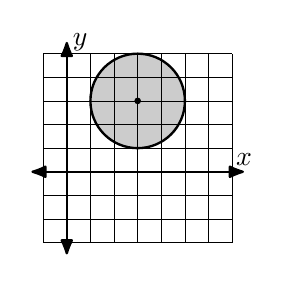
\begin{tikzpicture}[scale=0.3]

\filldraw [fill=\drawfill, line width=0.3mm] (3,3) circle (2);

\draw [line width=0.1mm] (-1,-3) grid (7,5);
 
\draw[line width=0.3mm, <->, >={Latex[round]}] (-1.5, 0) -- (7.5, 0);

\draw[line width=0.3mm, <->, >={Latex[round]}] (0, -3.5) -- (0, 5.5);

%\fill [opacity=.5,fill=\drawfill] (4,2) circle (2);

\fill [fill=black] (3,3) circle (4pt);

\node[anchor=south, inner sep=2pt, rotate=0] (x-label) at (7.5,0) {$ x$};  

\node[anchor=west, inner sep=2pt, rotate=0] (y-label) at (0,5.5) {$ y$};  

\end{tikzpicture} 
%2
\item 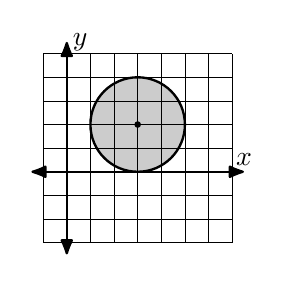
\begin{tikzpicture}[scale=0.3]

\filldraw [fill=\drawfill, line width=0.3mm] (3,2) circle (2);

\fill [fill=black] (3,2) circle (4pt);

\draw [line width=0.1mm] (-1,-3) grid (7,5);
 
\draw[line width=0.3mm, <->, >={Latex[round]}] (-1.5, 0) -- (7.5, 0);

\draw[line width=0.3mm, <->, >={Latex[round]}] (0, -3.5) -- (0, 5.5);

\node[anchor=south, inner sep=2pt, rotate=0] (x-label) at (7.5,0) {$ x$};  

\node[anchor=west, inner sep=2pt, rotate=0] (y-label) at (0,5.5) {$ y$};  

\end{tikzpicture} 
%3
\item 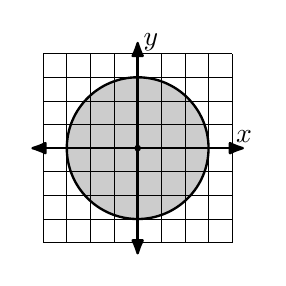
\begin{tikzpicture}[scale=0.3]

\filldraw [fill=\drawfill, line width=0.3mm] (0,0) circle (3);

\fill [fill=black] (0,0) circle (4pt);

\draw [line width=0.1mm] (-4,-4) grid (4,4);
 
\draw[line width=0.3mm, <->, >={Latex[round]}] (-4.5, 0) -- (4.5, 0);

\draw[line width=0.3mm, <->, >={Latex[round]}] (0, -4.5) -- (0, 4.5);

\node[anchor=south, inner sep=2pt, rotate=0] (x-label) at (4.5,0) {$ x$};  

\node[anchor=west, inner sep=2pt, rotate=0] (y-label) at (0,4.5) {$ y$};  

\end{tikzpicture} 
%4
\item 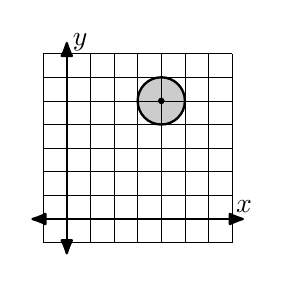
\begin{tikzpicture}[scale=0.3]

\filldraw [fill=\drawfill, line width=0.3mm] (4,5) circle (1);

\fill [fill=black] (4,5) circle (4pt);

\draw [line width=0.1mm] (-1,-1) grid (7,7);
 
\draw[line width=0.3mm, <->, >={Latex[round]}] (-1.5, 0) -- (7.5, 0);

\draw[line width=0.3mm, <->, >={Latex[round]}] (0, -1.5) -- (0, 7.5);

\node[anchor=south, inner sep=2pt, rotate=0] (x-label) at (7.5,0) {$ x$};  

\node[anchor=west, inner sep=2pt, rotate=0] (y-label) at (0,7.5) {$ y$};  

\end{tikzpicture} 
%5 
\item 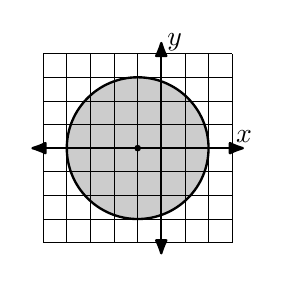
\begin{tikzpicture}[scale=0.3]

\filldraw [fill=\drawfill, line width=0.3mm] (-1,0) circle (3);

\fill [fill=black] (-1,0) circle (4pt);

\draw [line width=0.1mm] (-5,-4) grid (3,4);
 
\draw[line width=0.3mm, <->, >={Latex[round]}] (-5.5, 0) -- (3.5, 0);

\draw[line width=0.3mm, <->, >={Latex[round]}] (0, -4.5) -- (0, 4.5);

\node[anchor=south, inner sep=2pt, rotate=0] (x-label) at (3.5,0) {$ x$};  

\node[anchor=west, inner sep=2pt, rotate=0] (y-label) at (0,4.5) {$ y$};  

\end{tikzpicture} 
%6
\item 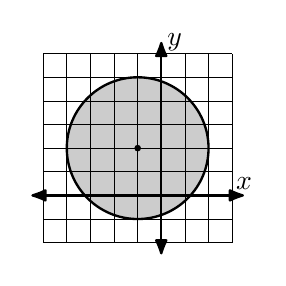
\begin{tikzpicture}[scale=0.3]

\filldraw [fill=\drawfill, line width=0.3mm] (-1,2) circle (3);

\fill [fill=black] (-1,2) circle (4pt);

\draw [line width=0.1mm] (-5,-2) grid (3,6);
 
\draw[line width=0.3mm, <->, >={Latex[round]}] (-5.5, 0) -- (3.5, 0);

\draw[line width=0.3mm, <->, >={Latex[round]}] (0, -2.5) -- (0, 6.5);

\node[anchor=south, inner sep=2pt, rotate=0] (x-label) at (3.5,0) {$ x$};  

\node[anchor=west, inner sep=2pt, rotate=0] (y-label) at (0,6.5) {$ y$};  


\end{tikzpicture} 
\end{multicols} 
\end{enumerate}  
%B
%\item \hspce 
%\begin{center}
%\vspace*{-2ex}
\scalebox{0.75}{
\noindent\begin{minipage}{\textwidth}
{
B. Find the center and radius of each circle with the given equation. 
\begin{enumerate}[label = \arabic*. ]
\begin{multicols}{2}
%1
\item \hspce $3x^2 + 3y^2 =12 $
%2
\item \hspce $x^2 + (y+4)^2 =81 $
%3
\item \hspce $(x-3)^2 + y^2 =144 $
%4
\item \hspce $(x+4)^2 + (y-3)^2 =64 $
%5 
%\item \hspce $(x-5)^2 + (y+1)^2 =49 $
\end{multicols} 
\end{enumerate}  
%C
%\item \hspce 
C. Write an equation of circle $C$ based on the given information. 
\begin{enumerate}[label = \arabic*. ]
%1
\item Center at (3, 2) and touching the x-axis 
%2
\item Center at (7, 5) and passing through (3, 4)
%3
\item Center at (4, 7) and passing through the origin 
%4
\item Center at (3, 7) and tangent to the y-axis
%5 
\item A circle with area 64 $\text{cm}^2 $ and center at (3, 6)
\end{enumerate}   

%D
%\item 
D. Write each equation of a circle in general form. 
\begin{enumerate}[label = \arabic*. ]
\begin{multicols}{2}
%1
\item \hspce  $(x-7)^2 + y^2 = 64$
%2
\item \hspce  $x^2 + (y+2)^2 = 49$
%3
\item  \hspce $(x+2)^2 + y^2 = 100$
%4
\item \hspce  $(x-5)^2 + (y-5)^2 = 27$
%5 
%\item \hspce  $(x+4)^2 + (y+4)^2 = 32$
\end{multicols} 
\end{enumerate}  

%E
%\item 
E. Transform each equation to standard form, then give the coordinates of the center and the radius. 
\begin{enumerate}[label = \arabic*. ]
\begin{multicols}{2}
%1
\item  $x^2 + y^2 -8x +2y -32 =0$
%2
\item   $x^2 + y^2 -6x -10y +18 =0$
%3
\item  $x^2 + y^2 - 6 x - 2 y - 15=0$
%4
\item  $x^2 + y^2 - 4 x + 6 y + 4 =0$
%5 
%\item \hspce $x^2 + y^2- 2 x  + 8 y - 47 =0$
\end{multicols} 
\end{enumerate}  

%\end{enumerate}  
}
\end{minipage}}
%\end{center}  

\end{frame}

\end{document}

